\documentclass{scrartcl}
\usepackage[ansinew]{inputenc}
%\usepackage[T1]{fontenc}
%\usepackage[ngerman]{babel} % Neue Rechtschreibung
\usepackage{amsmath} % Verbesserter Mathesatz
\usepackage{amssymb}
\usepackage{graphicx}

\parskip1ex
\title{\begin{small}Manual\end{small}\\Histogram-based background subtractor for ImageJ }
\date{January 2008 (rev. November 2010)}
\author{Janick Cardinale, \texttt{janick@inf.ethz.ch}, \\ MOSAIC Group, ETH Z�rich, www.mosaic.ethz.ch} 
\begin{document}

\maketitle

\section{Introduction}
\label{sec:intro}
To process images acquired using light microscopy systems, it is often useful to correct for inconstant background illumination and artifacts from autofluorescence. 
This software removes nonlinear background. The implemented algorithm is based on the assumption that, compared to the background region, object (foreground) regions are small. The plugin builds local histograms and assumes the most occuring intensity to be part of the background.

The plugin is is an alternative to deletion of low frequencies in Fourier space or the rolling ball algorithm (ImageJ standard implementation) proposed by S.Steinberg (1983). An example of the plugins functionality is shown in figure \ref{fig:alle2}.

\begin{figure}[h]
	\centering
		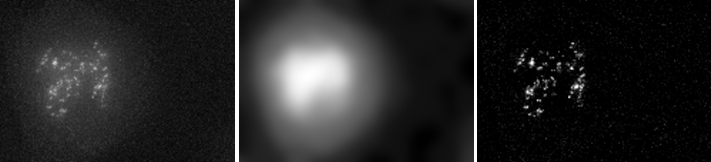
\includegraphics[width=0.90\textwidth]{images/alle2.png}
	\caption{Left: The original image A. Kinetochores are marked with a fluorescent protein. Middle: The generated background image B. Right: The final image with removed background illumination: C = A - B.}
	\label{fig:alle2}
\end{figure}


\section{Installation}
Copy the \texttt{mosaic\_plugins.jar} file to the ImageJs \texttt{plugins} directory. Then, restart ImageJ. The plugin can be launched from the \texttt{Mosaic} submenu in ImageJs plugin menu. 

The plugin handles 8-bit, 16-bit and 32-bit grayscale images or stacks. 

Prerequisits: At least Java 5.0 and ImageJ 1.36.

\section{How to use the plugin}
Open a grayscale image. Before starting the plugin, one might set a lower threshold using the \texttt{Ctrl-t} shortcut. This threshold can later be used to propose the plugins parameter. The lower intensity threshold should be set such that objects are above the threshold (and will be labelled red).

Start the plugin from the \texttt{Plugin} menu. Select the length parameter for your image: the parameter should be as small as possible but larger (in pixel) than any line that one can fit within the largest object in your image. 

If the autothreshold-algorithm (EM-algorithm) was successful or if you had manually selected a threshold before you launched the plugin, one might use the \texttt{propose parameter} button to get a automatically proposal for the histogram side length parameter. 

If you would like to get the background illumination image (the image that is subtracted from the original one), you can select the checkbox \texttt{show background image}. The background image (or image stack) will be shown after processing all the slices in a separate window.

There is no undo for this operation.

\section{Algorithm}
\subsection{Main algorithm}
A sliding window with side length $L$ is moved along the image with a speed of $L/2$ per iteration. At every iteration, the maximum of the local histogram (the histogram of the pixel intensities within the sliding window) is supposed to be background at the sliding windows position (center). For pixel where the background is not explicitly calculated, the background intensity is approximated by bi-linear interpolation of it's four nearest explicitly calculated pixel. A schematic overview of the algorithm is shown in figure \ref{fig:schema}.

\begin{figure}
	\centering
		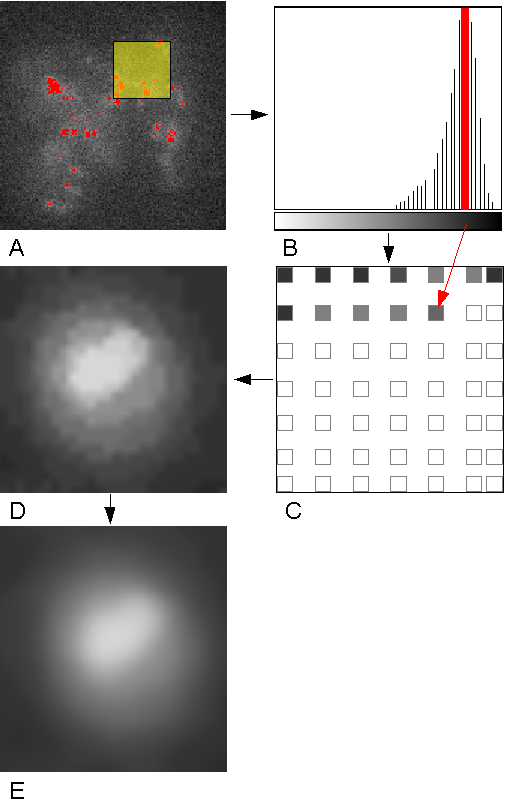
\includegraphics[width=0.50\textwidth]{images/BGSschema.png}
	\caption{A: The original image and the sliding window. B: The histogram of the pixel values within the sliding window. C: The background image in the first step: The pixel value at position of the middle of the sliding window is set to be equal to the mode of the histogram. D: Bilinear interpolation of the pixel that were not assigned a value in the first step. E: The smoothed background image after convolution with a Gaussian kernel.}
	\label{fig:schema}
\end{figure}

At the boundary of the image, the image is mirrored to generate the local histogram (Neumann boundary conditions).

In a second step, the created background image is convolved with a Gaussian kernel with a radius of $2\cdot L$ to filter for noise due to a too small $L$ or due to very high concentrations of objects.

\subsection{Proposal of the length parameter $L$}
A set of connected components $\mathcal{C}$ is generated using basic intensity based thresholding. Next, the largest diameter $d_{\textnormal{max}}$ that fits within any of the connected components in $\mathcal{C}$ is determined. The suggested parameter $L$ for the window size is double the size of $d_{\textnormal{max}}$.

\section{Disclaimer}
IN NO EVENT SHALL THE ETH BE LIABLE TO ANY PARTY FOR DIRECT, INDIRECT, SPECIAL, INCIDENTAL, OR CONSEQUENTIAL DAMAGES, INCLUDING LOST PROFITS, ARISING OUT OF THE USE OF THIS SOFTWARE AND ITS DOCUMENTATION, EVEN IF THE ETH HAS BEEN ADVISED OF THE POSSIBILITY OF SUCH DAMAGE. THE ETH SPECIFICALLY DISCLAIMS ANY WARRANTIES, INCLUDING, BUT NOT LIMITED TO, THE IMPLIED WARRANTIES OF MERCHANTABILITY AND FITNESS FOR A PARTICULAR PURPOSE. THE SOFTWARE PROVIDED HEREUNDER IS ON AN "AS IS" BASIS, AND THE ETH HAS NO OBLIGATIONS TO PROVIDE MAINTENANCE, SUPPORT, UPDATES, ENHANCEMENTS, OR MODIFICATIONS.

\end{document}

